\documentclass[]{report}

\newcommand{\sppath}[0]{../framework/}

% This file is a part of ShaperPerfect Article 2.0
% and entirely the property of Maxime Gaudin.
%
% 2011

% This file is a part of ShaperPerfect Article 2.0
% and entirely the property of Maxime Gaudin.
%
% 2011

% Execute #1 dans le shell disponible.
\newcommand{\shell}[1] {\immediate\write18{#1}}

% Execute #1 puis #2 si la commande a réussi, #3 sinon.
\newcommand{\shelltest}[3]{%
  \immediate\write18{#1 && touch witness}%
  \IfFileExists{witness}%
  {#2%
    \shell{rm witness 2>/dev/null}%
  }%
  {#3}%
}

% Exécute #2 si le package #1 est disponible.
\newcommand{\ifpackageavailable}[3]
{\shelltest{\sppath utils/findpackage.sh #1}{#2}{#3}}

% Affiche le message #1 dans la console lors de la compilation.
\newcommand{\infomessage}[1]
{\shell{\sppath utils/infomessage.sh "#1"}}

\newcommand{\fetchpackage}[1]
{
  \ifpackageavailable{#1}{}
  {
    \shell{\sppath utils/fetchlist.sh}
    \shell{\sppath utils/fetchpackage.sh #1}
  }
}

\newcommand{\safeusepackage}[1]
{
  \fetchpackage{#1}
  \usepackage{#1}
}

% This file is a part of ShaperPerfect Article 2.0
% and entirely the property of Maxime Gaudin.
%
% 2011

\newcommand{\spuselatex}[1]{
  \infomessage{LaTeX selected (#1).}
    \usepackage[utf8x]{inputenc}
    \usepackage[#1]{babel}
}

\newcommand{\spusexelatex}[1]{
 \ifpackageavailable{xunicode xltxtra fontspec polyglossia}
 {
  \infomessage{XeLaTeX selected.}
  	  \usepackage{xunicode}
  	  \usepackage{xltxtra}
  	  \usepackage{fontspec}
  	  \usepackage{polyglossia}
 
      \setdefaultlanguage{#1}
  	  \defaultfontfeatures{Mapping=tex-text}
  	  
  	  \newcommand{\og}{«}
  	  \newcommand{\fg}{»}
  }
  {}
}

\newcommand{\splanguage}[1]
{
  \ifpackageavailable{ifxetex}{
    \usepackage{ifxetex}

    \ifthenelse{\boolean{xetex}}{
      \spusexelatex{#1}
    }{
      \spuselatex{#1}
    }
  }
  { \spuselatex{#1} }

  \fetchpackage{float}  
  \fetchpackage{ifthen}
  \fetchpackage{xspace}
  \fetchpackage{relsize}
  \fetchpackage{algorithm2e}
  \usepackage[#1, boxruled, linesnumbered, vlined]{algorithm2e}
}


% This file is a part of ShaperPerfect Article 2.0
% and entirely the property of Maxime Gaudin.
%
% 2011

\ifpackageavailable{ifdraft} 
{
  \usepackage{ifdraft}

    \ifoptiondraft{
      \safeusepackage{draftwatermark}
      \SetWatermarkScale{5}
      \SetWatermarkText{\textbf{DRAFT}}
      \SetWatermarkLightness{0.90}
    }
    {} 
}
{\infomessage{Draft support disabled.}}


% This file is a part of ShaperPerfect Article 2.0
% and entirely the property of Maxime Gaudin.
%
% 2011

\bibliographystyle{alpha}

% Sample 
% \newglossaryentry{sample}{name={sample}, description={A sample entry}}
\newglossaryentry{backface_culling}{name={backface culling}, 
description={(Abattage?) Appelé aussi simplement \eng{culling}, c'est
l'opération consistant à éliminer toutes les faces faisant dos à la caméra et
ne pouvant par conséquent pas être vues.}}

\newglossaryentry{motion_blur}{name={motion blur}, 
description={(Flou de mouvement) C'est le flou généré par une vitesse
d'obturation de la caméra trop grande. }}

\newglossaryentry{clipping}{name={clipping},
description={C'est l'élimination des face hors du champ de la caméra.}}

\newglossaryentry{aliasing}{name={aliasing},
description={Le crénelage sur une image.}}

\newglossaryentry{supersampling}{name={supersampling},
description={Littéralement, sur-échantillonnage, cette technique permet
d'éviter des effets d'aliasing.}}

\newglossaryentry{jittering}{name={jittering},
description={C'est la perturbation que les rayons lumineux subissent
lorsqu'une surface mal polie les réfléchi (par exemple du verre sablé).}}

\newglossaryentry{adaptative_sampling}{name={adaptative sampling},
description={C'est une forme de supersampling qui n'est réalisée que si un
certain seuil d'aliasing est détecté.}}

\newglossaryentry{shader}{name={shader},
description={Un shader est un programme appliqué à l'ensemble des pixel ou des
sommets des polygones de la scène. Ils sont aujourd'hui incorporés dans le
pipeline de rendu des cartes graphiques.}}


% This file is a part of ShaperPerfect Article 2.0
% and entirely the property of Maxime Gaudin.
%
% 2011

\newcommand{\tsl}[1]{\textsl{#1}}
\newcommand{\tbf}[1]{\textbf{#1}}
\newcommand{\ttt}[1]{\texttt{#1}}
\newcommand{\tsc}[1]{\textsc{#1}}

\newcommand{\ie}{\textsl{i.e.}\ }
\newcommand{\cf}{\textsl{Cf.}\ }
\newcommand{\etc}{\textsl{etc.}}
\newcommand{\eg}{\textsl{e.g.}\ }

\newcommand{\resp}{\textsl{resp.}\ }

\newcommand{\wrt}{\textsl{w.r.t.}\ }
\newcommand{\Wrt}{\textsl{W.r.t.}\ }

% This file is a part of ShaperPerfect Article 2.0
% and entirely the property of Maxime Gaudin.
%
% 2011

\safeusepackage{pifont}
\newcommand{\tickmark}{\textcolor{green}{\ding{51}}}
\newcommand{\tackmark}{\textcolor{red}{\ding{55}}}
\newcommand{\tuckmark}{\textcolor{orange}{\textbf{?}}}

% This file is a part of ShaperPerfect Article 2.0
% and entirely the property of Maxime Gaudin.
%
% 2011

\usepackage{amsfonts}
\usepackage{amsmath}
\usepackage{amsthm}

% This file is a part of ShaperPerfect Article 2.0
% and entirely the property of Maxime Gaudin.
%
% 2011

\usepackage{multicol}
\usepackage{varioref}
\usepackage{ifthen}

\safeusepackage{float}
\safeusepackage{todonotes}
\safeusepackage{lipsum}

\ifpackageavailable{pdflscape}
{\usepackage{pdflscape}}
{\usepackage{lscape}}

\def\texcapitalize#1#2/{{\uppercase{}#2}}
\newcommand{\capitalize}[1]{\texcapitalize#1/}

% This file is a part of ShaperPerfect Article 2.0
% and entirely the property of Maxime Gaudin.
%
% 2011

\newcommand{\customdate}[0]{
  \ifpackageavailable{datetime} 
  {
    \usepackage{datetime}
    \newdateformat{customdateformat}{\monthname[\THEMONTH] \THEYEAR}
    \date{\customdateformat\today}
  }
  {\date{\today}}
}


\input{\sppath latex/hyperref}
% This file is a part of ShaperPerfect Article 2.0
% and entirely the property of Maxime Gaudin.
%
% 2011

\ifpackageavailable{minted} {
  \shelltest{\sppath utils/findbin.sh pygmentize}{
    \usepackage{minted}
    \newcommand{\inputcode}[3][] { \inputminted[####1]{####2}{####3} }
  }{}
}
{
  \infomessage{Minted listings support disabled.}
 
  \newcommand{\inputcode}[2] {
    \ifpackageavailable{pdftexcmds}{}
    {\fetchpackage{oberdiek}}

    \fetchpackage{xcolor}
  
    \usepackage{listingsutf8}
    \usepackage{xcolor}
    \definecolor{colKeys}{rgb}{0,0,1}
    \definecolor{colIdentifier}{rgb}{0,0,0}
    \definecolor{colComments}{rgb}{0,0.6,0.1}
    \definecolor{colString}{rgb}{0.6,0.1,0.1}
    
    \lstset{%
    	float=hbp,% 
    	basicstyle=\ttfamily\small, % 
    	identifierstyle=\color{colIdentifier}, % 
    	keywordstyle=\color{colKeys}, % 
    	stringstyle=\color{colString}, % 
    	commentstyle=\color{colComments}, % 
    	columns=flexible, % 
    	tabsize=2, % 
    	frame=trBL, % 
    	%frameround=tttt, % 
    	extendedchars=true, % 
    	showspaces=false, % 
    	showstringspaces=false, % 
    	numbers=left, % 
    	numberstyle=\tiny, % 
    	stepnumber=2,%
    	breaklines=true, % 
    	breakautoindent=true, % 
    	captionpos=b,% 
    	xrightmargin=-1cm, % 
    	xleftmargin=-1cm, %
    	inputencoding=utf8
    }
    
    \lstset{
    	literate=	{é}{{\'e}}1
    			{è}{{\`e}}1
    			{ê}{{\^e}}1
    			{à}{{\`a}}1
    			{ù}{{\`u}}1
    			{ë}{{\"e}}1
    			{ô}{{\^o}}1
    } 
    \lstinputlisting[language=##1]{##2}
  }
}
{\infomessage{UTF8 listings support disabled.}}



\splanguage{french}
\usepackage{float}
\usepackage{tikz}
\usetikzlibrary{shapes.multipart} 

\newcommand{\eng}[1]{\tsl{#1}}

\newcommand{\raytracing}[0]{\eng{raytracing}}
\newcommand{\remark}[1]{

\vspace*{1em}\hspace*{\fill}\begin{minipage}{.8\textwidth}
\it\tbf{Remarque :} #1
\end{minipage}
}
\safeusepackage{wasysym}

\newcommand{\gfont}{%
	\fontencoding{\encodingdefault}%
	\fontfamily{ptm}%
	\fontseries{bc}%
	\fontshape{bf}%
	\fontsize{65}{60}%
	\selectfont}

% \quote[Auteur]{Citation}
\renewcommand{\quote}[2][null]
{%
	~\\
	\begin{minipage}{\textwidth}%
	\vspace*{\baselineskip}
		\parbox{0.2\textwidth} {\textcolor[rgb]{0.5,0.5,0.5}{\gfont "}}%
			\parbox{0.8\textwidth}%
			{%
				\textcolor[rgb]{0.3, 0.3, 0.3}{\textsl{#2}}%
				\ifthenelse{\equal{#1}{null}}{}{\begin{flushright}\textsc{#1}\end{flushright}}%
			}%
	\end{minipage}%
}

\usepackage{subfigure}
\usepackage{wrapfig}

\usepackage{titlesec}
\titlespacing{\paragraph}
{0pt}
{0.5\baselineskip}
{.35em}


\title{\tbf{Projet personnel en Informatique\\ Lyon Ray Tracer}}
\author{%
Maxime \tsc{Gaudin}\\
~\\
\small \href{mailto:maxime.gaudin@polymtl.ca}{maxime.gaudin@polymtl.ca}\\
\small Institue National des Sciences Appliquées de Lyon (INSA)\\
\small École Polytechnique de Montréal
}
\customdate

\begin{document}
\maketitle

\begin{abstract}
  Le projet personnel nous permet de réaliser, sous la direction d'un
  professeur du département, un programme de recherche dans le domaine qui
  nous convient. C'était donc pour moi une opportunité de me lancer dans le
  développement d'un algorithme aussi puissant que mystérieux : Le
  \raytracing{}. Et c'est en l'honneur de ma ville natale, Lyon (France), j'ai nommé ce
  programme \tsl{Lyon Ray Tracer}.\\
  
  Ce rapport vous permettra d'avoir une vue d'ensemble sur le
  travail que j'ai effectué.
\end{abstract}
 % CHECKED

\section{Introduction}
Dans un monde où l'informatique et la virtualisation des environnements de
travail est omniprésente, la visualisation des données est devenu un enjeux
primordiale pour des domaines aussi variés que la médecine, l'architecture,
l'industrie du jeux vidéo ou encore les interfaces utilisateur.

\paragraph{\eng{Rasterisation}}
Encore aujourd'hui, la méthode privilégiée de visualisation des environnements
3D est la \eng{rasterisation}. Cette technique consiste à modéliser
l'\tsl{univers}\footnote{Au sens mathématique, \ie tout ce qui est contenu
dans un système en troi dimensions.} par un ensemble de triangles. Ces
triangles sont transformé (\ie translatés, mis à l'échelle, \etc) puis projeté
dans un monde plan : Notre écran. La \fref{rasterisationPipeline} représente
grossièrement le cheminement des données jusqu'à l'image finale.

\begin{figure}[H]
\begin{center}
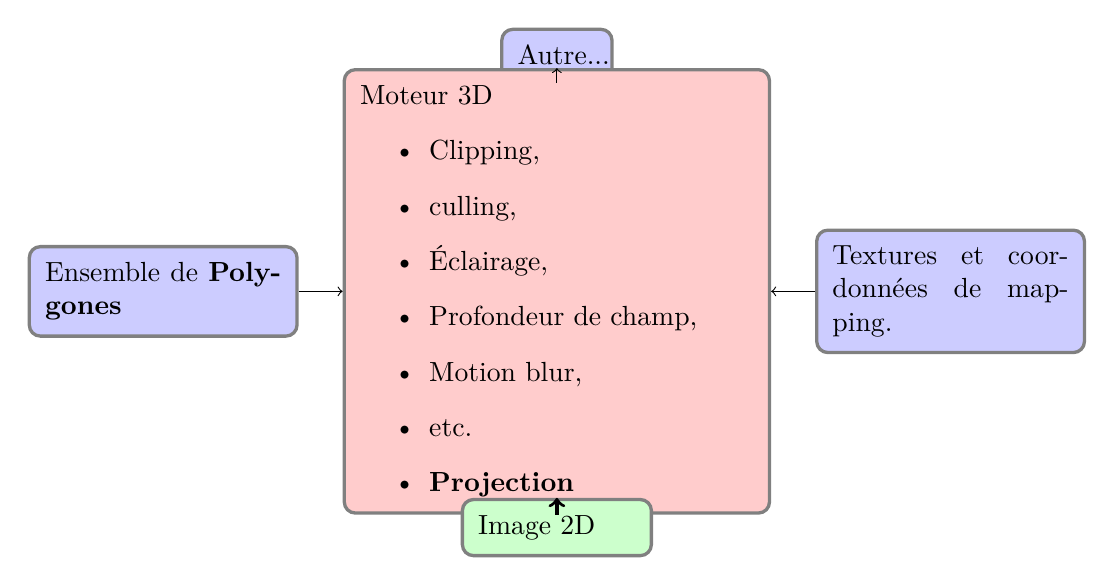
\begin{tikzpicture}
  [entree/.style={
    draw=black!50,
    fill=blue!20,
    rectangle,
    rounded corners,
    inner sep=.2cm,
    very thick}, systeme/.style={
    draw=black!50,
    fill=red!20,
    rectangle,
    rounded corners,
    inner sep=.2cm,
    very thick}, sortie/.style={
    draw=black!50,
    fill=green!20,
    rectangle,
    rounded corners,
    inner sep=.2cm,
    very thick}]

  \node [entree] at (-5,0) (polygone) {
  \begin{minipage}{3cm}
    Ensemble de \textbf{Polygones}
  \end{minipage}
  };

  \node [entree] at (5,0) (textures) {
  \begin{minipage}{3cm}
    Textures et coordonnées de mapping.
  \end{minipage}
  };

  \node [entree] at (0,3) (other) {
  \begin{minipage}{1cm}
    Autre...
  \end{minipage}
  };

  \node [systeme] (engine) {
  \begin{minipage}{5cm}
    Moteur 3D 
    \begin{itemize}
      \item Clipping,
      \item culling,
      \item Éclairage,
      \item Profondeur de champ,
      \item Motion blur,
      \item etc.
      \item \textbf{Projection}
    \end{itemize}
  \end{minipage}
  };

  \node [sortie] at (0,-3) (image) {
  \begin{minipage}{2cm}
    Image 2D
  \end{minipage}
  };

  \draw [->] (polygone) -- (engine);
  \draw [->] (textures) -- (engine);
  \draw [->] (other) -- (engine);
  \draw [very thick, ->] (engine) -- (image);
\end{tikzpicture}
\caption{Représentation grossière du pipeline de rendu via la
rasterisation\label{rasterisationPipeline}}
\end{center}

\end{figure}


L'avantage de cette technique vient du fait que les calculs sont très
aisément parallélisables. Nous assistons d'ailleurs à un développement de
technologie dans ce sens : Les \gls{GPU} sont devenu de vraies collections de
processeurs.

\newpar Mais cette technique n'offre pas que des avantages. En effet, la
compleification des scènes en 3D et surtout la demande du publique pour des
rendu encore plus réaliste pousse dans ses retranchement le matériel et les
logiciels de visualisation 3D. Mais depuis quelques plus de 30 ans
\cite{Whitted1980}, chercheurs et ingénieurs développent une technique de
rendu simple mais très puissante : Le \raytracing !

\subsection{Le \raytracing ?}

\subsection{Objectifs du projet}
Les objectifs du projet sont nombreux, aussi bien sur le plan de
l'architecture logiciel, que de la gestion de projet ou encore u
développement.

\paragraph{Architecture logiciel}
Un des buts principal du projet (si ce n'est le but principal du projet) est
de créer un programme ouvert à l'extension et pouvant servir de base à la
création d'un \raytracing plus évolué, ou plus rapide, ou plus facile à
utiliser, etc.

\paragraph{Portabilité}
Afin d'être le plus portable possible, j'ai décidé d'utiliser un mélange
d'outils standards comme :
\begin{itemize}
  \item C/C++ : Compilable sur presque toutes les plateformes.
  \item Les autotools\footnote{\url{http://sources.redhat.com/autobook/}} :
  Système de build standard et ne nécessitant aucun autre programme que make
  et bash.
  \item Boost : La bibliothèque C++ de référence.
  \item libpng/libjpg : Pour l'import texture et l'export des résultats.
  \item lib3ds : Pour l'importation des modèles 3D.
\end{itemize}

\paragraph{Gestion de projet}
J'ai réalisé ce projet seul du 24 Septembre au 1 Décembre en utilisant un
style de développement \gls{XP}\footnote{\url{http://www.extremeprogramming.org/}}.
Le gestionnaire de version utilisé est git et le projet ainsi que son
\href{http://digitalguru.github.com/LyonRayTracer}{site web} sont hébergés sur
GitHub.

\paragraph{Implémentation}
Il était pour moi primordial de respecter tout au long de ce projet des
\eng{guidelines} afin d'assurer une cohérence de tout le code (de plusieurs
miliers de lignes tout de même). La documentation fait aussi partie intégrante
du processus de développement et la génération de celle-ci fait partie du
\eng{pipeline} de compilation.

\paragraph{Fonctionnalité du ray tracer}
Reprenons les objectifs fixés dans le sujet :
\begin{enumerate}
  \item Un moteur de \raytracing ``classique''.\textcolor[rgb]{0.0, 0.9, 0.2}{\checkmark}
  \item La gestion de primitives (sphères, plan, tores, et en général toutes
    les figures ayant une représentation paramétrique).\textcolor[rgb]{0.0, 0.9, 0.2}{\checkmark}
  \item La gestion de plusieurs types de caméras : Orthographique,
    perspective, \etc\textcolor[rgb]{0.0, 0.9, 0.2}{\checkmark}
  \item La gestion de plusieurs types de lumières : Point, plan, sphérique,
    \etc.\textcolor[rgb]{0.0, 0.9, 0.2}{\checkmark}
  \item La gestion d'au moins un format de représentation polygonale.\textcolor[rgb]{0.0, 0.9, 0.2}{\checkmark}
  \item La mise en place des structures accélératrices.\textcolor[rgb]{0.0, 0.9, 0.2}{\checkmark}
\end{enumerate}

\newpar J'ai aussi pris le temps d'implémenter :
\begin{enumerate}
  \item Un chargeur de scènes XML.
  \item La lecture et l'écriture d'images au format PNG ou JPG (avec la
  possibilité d'ajouter d'autre formats).
  \item La gestion des textures.
  \item Le \gls{supersampling}.
\end{enumerate}

\subsection{Non-objectifs}
Comme dans tout projet, celui-ci possède des non-objectifs, \ie des objectifs
que j'ai décider volontairement de ne pas atteindre, ou en tout cas de ne pas
viser. 

\newpar D'abord, la vitesse d'exécution. Les \eng{raytracers} commerciaux sont
de réelles prouesses d'ingénierie et d'optimisation et j'ai considérer que
l'optimisation de tels programme sort du contexte d'un projet personnel.
 % CHECKED

\chapter{Objectifs}
Les objectifs du projet sont nombreux, aussi bien sur le plan de
l'architecture logiciel, que de la gestion de projet, de la rédaction ou
encore du développement.

\paragraph{Architecture logiciel -} Un des principaux buts du projet (si ce
n'est le but principal du projet) est de créer un programme ouvert à
l'extension et pouvant servir de base à la création d'un \eng{raytracer}\ plus
évolué, plus rapide, ou plus facile à utiliser.

L'architecture du programme est défini à la section \ref{sec:architecture}.

\paragraph{Portabilité -} Afin d'être le plus portable possible, j'ai décidé
d'utiliser un ensemble d'outils standards et libres :
\begin{itemize}
  \item \tsl{Le langage C++ :}\ \eng{Open-Spec}\ et compilable sur presque
    toutes les plateformes.
  \item \tsl{Les autotools}\footnote{\url{http://sources.redhat.com/autobook/}
    :}\ Système de build standard et ne nécessitant aucun autre programme que
    make et bash. De plus, il assure une portabilité maximale en vérifiant la
    présence de toutes les bibliothèques nécessaire à la compilation et au bon
    fonctionnement du programme.
  \item \tsl{Boost :}\ La bibliothèque C++ de référence.
  \item \tsl{libpng/libjpg :}\ Pour l'import texture et l'export des résultats.
  \item \tsl{lib3ds :}\ Pour l'importation des modèles 3D.
  \item \tsl{\LaTeX{} :}\ Pour la rédaction du rapport.\\

  \item \tsl{Tim Horton :}\ Pour le café et les beignets.
\end{itemize}

\paragraph{Gestion de projet -} J'ai réalisé ce projet seul du 24 Septembre au
1 Décembre en utilisant un style de développement
\gls{XP}\footnote{\url{http://www.extremeprogramming.org/}}.  Le gestionnaire
de version utilisé est \tsl{git}\ et le projet ainsi que son
\href{http://digitalguru.github.com/LyonRayTracer}{site web} sont hébergés sur
\href{http://github.com}{GitHub}.

\remark{Parce que la charge de travail aurait été trop grande, j'ai décidé de
ne pas rédiger les documents de références du type \tsl{Dossier
d'initialiation}, \tsl{Dossier de jalonnage}, \tsl{Planning prévisionnel},
\etc J'ai cependant pris soin de rédiger une documentation exhaustive de
chacune des classes du projet.}
\vspace*{1em}

\paragraph{Implémentation -} Il était pour moi primordial de respecter tout au
long de ce projet des \eng{guidelines}\ afin d'assurer une cohérence de tout
le code (plusieurs milliers de lignes tout de même). J'ai pour cela suivit
principalement le guide de style définit par Herb \tsc{Sutter} dans
\cite{Sutter05}. Je me suis aussi inspiré de \cite{Meyers94}.\\

Enfin, la documentation fait aussi partie intégrante du processus de
développement et la génération de celle-ci fait partie du \eng{pipeline} de
compilation.

\paragraph{Fonctionnalité du ray tracer -} Reprenons les objectifs fixés dans
le sujet :
\begin{enumerate}
  \item \tickmark{} Un moteur de \raytracing\ ``classique''.
  \item \tickmark{} La gestion de primitives (sphères, plan, boite,
    triangles).
  \item \tickmark{} La gestion de plusieurs types de caméras : Orthographique,
    perspective, \etc
  \item \tickmark{} La gestion de plusieurs types de lumières : Point, plane,
    directionnelle, \etc
  \item \tickmark{} La gestion d'au moins un format de représentation
    polygonale.
  \item \tickmark{} La mise en place des structures accélératrices.
  \item \tackmark{} La gestion du \eng{photon mapping} : Comme je l'avais
    pressentie dans mon sujet, le temps alloué au projet était insuffisant
    pour l'implémentation d'une telle fonctionnalité.\\
\end{enumerate}

J'ai cependant pris le temps d'implémenter en plus :
\begin{enumerate}
  \item Un chargeur de scènes XML.
  \item La lecture et l'écriture d'images au format PNG ou JPG (avec la
    possibilité d'ajouter d'autre formats).
  \item La gestion des textures.
  \item Le \gls{supersampling}.
  \item La gestion des ombres douces.
  \item La gestion de la profondeur de champ.
\end{enumerate}

\subsection{Non-objectifs}
Comme dans tout projet, celui-ci possède des non-objectifs, \ie des objectifs
que j'ai volontairement choisi de ne pas atteindre, ou en tout cas de ne pas
viser.\\

D'abord, concernant la vitesse d'exécution. Les \eng{raytracers} commerciaux
sont de réelles prouesses d'ingénierie et d'optimisation et j'ai considéré que
l'optimisation de mon programme sortait du contexte d'un projet personnel.\\

Il ne s'agissait pas non plus d'en faire un produit fini mais plutôt un
\tsl{proof of concept}. Il reste donc de nombreuses améliorations tant au
niveaux des fonctionnalités existantes qu'au niveau de celles à ajouter.
 % CHECKED
 % CHECKED

\section{État de l'art}
Il est hélas impossible de réaliser un état de l'art complet sur le
\raytracing car cela nécessiterais des mois de recherche et mériterait un
papier complet sur le sujet\footnote{Je vous invite à consulter
\cite{Wald01stateof}}. Nous pouvons cependant retracer les grandes dates
de cette technologie et tenter d'apercevoir les perspectives de celle ci.

\paragraph{Invention}

 % CHECKED

\section{Architecture}
C'est la partie la plus importante de mon programme. 


\chapter{Résultats \& Analyse}
Afin que le rapport reste dans des proportions raisonnables, je n'aborderai
pas tous les résultats que j'ai obtenu. Je vous invite donc à ``jouer'' avec
le programme et essayer les quelques scènes d'exemples.

\clearpage
\section{Gestionnaire de scènes\label{scenemanager}}
Un des élément principaux, il permet grâce à une description textuelle, de
générer la représentation mémoire de la scène. C'est par conséquent
l'interface de communication entre l'utilisateur et le client.

La démocratisation et la facilité du langage XML m'ont poussé à le choisir
comme métalangage de description. De plus, la disponibilité d'outils pour le
\eng{parser}\ rend son utilisation beaucoup plus simple\footnote{Dans mon cas,
la \tsl{parsing}\ est assuré par \tsl{Boost}\ ce qui le rend très solide.}.

Enfin, il augmente l'interopérabilité avec d'autre logiciel comme les
modeleurs par exemple.

\subsection{Exemple} 
La code suivant est un exemple simple de scène mettant en jeu 3 sphères, 1 plan
et une caméra avec gestion de la profondeur de champ :

\inputcode{xml}{../../code/scenes/DOF.lrt}

Comme ci-dessus, une description de scène est composée de 4 blocs :
\begin{enumerate}
  \item Un nœud \ttt{camera} : C'est ici qu'est déclaré l'\tsl{unique}\ caméra
  de la scène.
  \item Un nœud \ttt{materials} : C'est ici que doivent être déclaré l'ensemble
  des matériaux identifiés par une chaine de caractère \tsl{unique}.
  \item Un nœud \ttt{lights}.
  \item Un nœud \ttt{geometries}.
\end{enumerate}
\remark{L'ordre n'est pas imposé.}\vspace*{1em}

Comme précisé dans l'architecture, c'est chaque \eng{builder}\ qui décrit les
paramètres dont il a besoin pour fonctionner. Certains sont obligatoires,
d'autres optionnels.

\subsection{Améliorations}
\begin{description}
  \item [Gestion de la casse] Pour l'instant, la détection des paramètres est
    \tsl{case-sensitive}, c'est inutile et source d'erreurs difficiles à
    débusquer.
\item [Auto-description] Chaque \tsl{builder}\ devrait pouvoir se décrire via
  la ligne de commande en expliquant quels sont les paramètres dont il a
  besoin et leurs domaines de définitions.
\end{description}

Ces deux améliorations sont relativement simples à implémenter et c'est
principalement le développement d'autres fonctionnalité et le manque de temps
qui m'ont empêcher de les ajouter au programme. 

Il faut tout de même noter que la seconde amélioration n'avait pas été prévu
et qu'il faudra par conséquent changer l'interface des \tsl{builder}, ce qui impacte
l'ensemble de code existant.  C'est donc un oubli très gênant de ma part.

\subsection{Bug connu}
Aucun.
 % CHECKED

\clearpage
\section{Journalisation}
Pour un programme d'une telle ampleur, il est important de pouvoir retracer le
l'exécution sans avoir à utiliser un debugger. C'est pourquoi j'ai choisi de
me tourner vers une gestion centralisée et systématique des logs.

\subsection{Exemple :} Rendu de la scène \ttt{DOF.lrt} 
\begin{center}
\begin{verbatim}
[Core] - Builders discovering...
[SceneReader] - 'material' builder added.
[SceneReader] - 'perspective' builder added.
[SceneReader] - 'perspectiveDOF' builder added.
[SceneReader] - 'point' builder added.
[SceneReader] - 'area' builder added.
[SceneReader] - 'sphere' builder added.
[SceneReader] - 'plane' builder added.
[SceneReader] - 'mesh' builder added.
[Core] - Building scene...
[SceneReader] - Reading scene : scenes/DOF.lrt ...
[SceneReader] - Image...
[Image] - Building new output frame (600, 600)... OK
[SceneReader] - Camera...
[PerspectiveDOF] - New Camera : Eye - ( 0 ,0 ,8 ), LookAt - ( 0 ,0 ,0 ),
Direction ( 0 ,0 ,-1 )
[SceneReader] - Materials...
[MaterialBuilder] - New material with diffuse = [ R=1, G=0, B=0 ].
[MaterialBuilder] - New material with diffuse = [ R=1, G=1, B=0 ].
[MaterialBuilder] - New material with diffuse = [ R=0, G=1, B=0 ].
[MaterialBuilder] - New material with diffuse = [ R=0, G=0, B=1 ].
[SceneReader] - Lights...
[SphereBuilder] - New point light at ( -20 ,20 ,20 )
[SceneReader] - Geometry...
[SphereBuilder] - New sphere at ( 0 ,0 ,0 ) (radius = 1)
[SphereBuilder] - New sphere at ( -1 ,0 ,4 ) (radius = 1)
[SphereBuilder] - New sphere at ( 2 ,0 ,-4 ) (radius = 1)
[PlaneBuilder] - New plane at ( 0 ,-1.2 ,0 ) (normal= ( 0 ,1 ,0 ))
[Core] - Rendering...

0%...........................................................
10%...........................................................
20%...........................................................
...
100%..........................................................
[Core] - Saving...
[Core] - Cleanup...
\end{verbatim}
\end{center}

\subsection{Améliorations}
\begin{description}
  \item [Gestion des niveaux d'alerte] Alors que certaines informations
    peuvent être utiles à l'utilisateur, d'autres sont purement fonctionnelles
    et permettent un débugage plus rapide. Il serait donc judicieux de pouvoir
    affecter des niveaux aux événements de journalisation dans le but de
    pouvoir les filtrer.
\end{description}

\subsection{Bug connu} 
Aucun.
 % CHECKED

\clearpage
\section{Texture}
Le plaquage des textures est intimement lié à la géométrie en question. Le
moteur ne fait donc que très peu de travail comparé à la géométrie qui doit
projeter elle même la texture et donner, en fonction des informations de
collisions, la couleur au point demandé. 

\remark{Comme nous pouvons le voir dans le description de l'architecture,
la gestion des différents formats d'image n'est pas à la charge
de la géométrie.}

\subsection{Exemple}
La \tsl{fig. \ref{fig:texture}} présente un exemple de plaquage de texture
(ici, une grille en metal) sur une sphère.

\begin{figure}[h]
  \begin{center}
    \includegraphics[width=.5\textwidth, keepaspectratio=true]{../../diary/17.png}
    \caption{Un exemple de rendu avec plaquage de texture\label{fig:texture} sur
    une sphère.}
  \end{center}
\end{figure}

\subsection{Amélioration \& bug connu}
Aucun.
 % CHECKED

\clearpage
\definecolor{bg}{rgb}{0.95,0.95,0.95}
\section{Réflexion}
Fonctionnalité de base, le calcul du rayon réfléchi est relativement simple :
\begin{center}
  \inputcode[bgcolor=bg]{c++}{code/reflection.cc}
\end{center}

Le schéma de la \tsl{fig. \ref{fig:reflectionSchema}} illustre bien ce calcul. 
\begin{figure}[h]
  \begin{center}
    \includegraphics[width=.7\textwidth,
    keepaspectratio=true]{img/reflectionSchema}
    \label{fig:reflectionSchema}
  \end{center}
\end{figure}

\subsection{Exemple}
La \tsl{fig. \ref{fig:reflection}} présente un exemple de reflexion sur une
sphère.

\begin{figure}[h]
  \begin{center}
    \includegraphics[width=\textwidth, keepaspectratio=true]{../../diary/10.png}
    \caption{Un exemple du rendu de la réflexion de l'environnement sur une
    sphere\label{fig:reflection}}
  \end{center}
\end{figure}

\subsection{Amélioration \& bug connu}
Aucun.
 % CHECKED

\clearpage
\section{Réfraction}
Le calcul du rayon réfracté est un peu plus compliqué :
\begin{center}
\inputcode[bgcolor=bg]{c++}{code/refraction.cc}
\end{center}

D'un part, il faut déterminer si le rayon est entrant ou sortant. Pour cela,
je compare la direction de la normale avec le rayon incident. Si les deux
rayons sont de même sens alors le rayon est entrant.\footnote{Pour se
convaincre du calcul de \ttt{input}, un simple dessin suffit.} Sinon il est
sortant.

Avant de calculer le rayon réfracté, nous devons vérifier que l'angle entre
la normal et le rayon incident ne dépasse pas l'angle maximale de réfraction.
Autrement dit, si le rayon est rasant, il y a réflexion totale.

Enfin, le calcul du rayon absorbé est fait selon la loi de Snell-Descartes :
$$n_1.\sin(\theta_1) = n_2.\sin(\theta_2)$$

\subsection{Exemple}
\begin{figure}[h]
  \includegraphics[width=\textwidth, keepaspectratio=true]{../../diary/09.png}
  \caption{Un exemple du rendu de la réfraction de l'environnement sur une
  sphere}
\end{figure}

\subsection{Amélioration \& bug connu}
Aucun.
 % CHECKED

\clearpage
\section{Interpolation des normales}
Comme nous pouvons le voir sur la \tsl{fig.\ref{fig:angel}}, l'utilisation
brute des
normales fournit par le modeleur ne nous permet pas d'obtenir un résultat très
esthétique. En effet, chaque face possède une normale et la transition entre
deux triangles est très marquée.\\

La solution consiste à assigner non pas une normale par face, mais 3 : une
pour chaque sommet. Ainsi, en moyennant la normale de chaque sommet en
fonction des faces auxquelles elle appartient, nous pourrons interpoler la
normale au point d'intersection en prenant maintenant en considération les
faces alentours. La \tsl{fig. \ref{fig:smoothnormal}}\ montre le résultat
obtenu.

\paragraph{Les coordonnées barycentriques}
\begin{wrapfigure}{r}{.5\textwidth}
  \includegraphics[width=.4\textwidth,
  keepaspectratio=true]{img/barycentricCoordinates}
  \label{fig:barycentric}
\end{wrapfigure}
Toute la difficulté de l'interpolation des normales repose donc sur la
pondération des différentes normales de la face. Pour cela, il est nécessaire
de passer en coordonnées barycentriques. Dans ce système, les coordonnées du
point d'intersection sont exprimées en fonction de deux côtés du triangle
comme le montre la \tsl{fig. \ref{fig:barycentric}}.\\

Il est alors évident de calculer le poids de chaque normal à la normal au
point d'intersection :
$$\vec{N} = N_a + a * (N_b - N_a) + b * (N_c - N_a)$$
où $a = |AB|$, $b = |AC|$ et $N_a$ (\resp $N_b$ et $N_c$) est la normale en
$A$ (\resp $B$ et $C$).

\subsection{Exemple}
\begin{figure}[h]
  \includegraphics[width=\textwidth, keepaspectratio=true]{../../diary/16.png}
  \caption{Un exemple de rendu avec interpolation des normales\label{fig:smoothnormal}}
\end{figure}

\subsection{Amélioration}
\begin{description}
  \item [Génération des normales] Afin de réduire la complexité de
    l'importeur, j'ai laissé le calcul des normals par sommet à un programme
    externe. Il serait judicieux (et pas vraiment compliqué) d'intégrer le
    lissage au processus de chargement normal.
\end{description}

\subsection{Bug connu}
Aucun.
 % CHECKED

\clearpage
\section{Mesh}
Un \eng{mesh} n'est en réalité qu'un ensemble de triangle, de texture et de
coordonnées de textures. Ce n'est donc pas dans l'agrégation que se situe la
difficulté.\\

Le vrai problème se trouve dans le nombre de triangles qu'un mesh peut
contenir. Sans structure accélératrice, le calcul de chaque pixel devrait
tester l'intersection avec tout les triangles. C'est inimaginable et le temps
de la calcul serait multiplié par le nombre de triangles de la scène (certains
de mes modèles possèdent plus de 80 000 faces).

\subsection{L'\tsl{octree}}
Pour optimiser les calculs d'intersection, j'ai décidé d'utiliser une structure
appelée \tsl{Octree}. Cette structure permet de diviser l'espace et de le
représenter par un arbre. Son fonctionnement est relativement simple :
\begin{description}
  \item [\tbf{Initialisation}] Lors de la création, trouver le cube englobant
    tous les triangles du \eng{mesh}. Puis, récursivement, diviser ce cube en
    8 cubes (au maximum), chacun moitié du cube existant. Continuer tant que
    le contenu du cube courant est supérieur au contenu maximal. Après cette
    étape, nous nous retrouvons avec une subdivision du type de celle
    représenté à la \tsl{fig. \ref{octree}}.
  \item [\tbf{Calcul d'intersection}] D'abord, vérifier que le rayon
    intersecte le cube englobant. Puis, pour chacun de ses cubes enfant,
    établir la collision.\footnote{Il est possible d'accélérer le résultat en
    tenant compte de la direction du rayon sortant lors de l'intersection avec
    un cube.} Prendre le plus prêt et descendre comme ceci jusqu'à
    un cube feuille. Enfin tester l'intersection avec les triangle de la
    feuille.
\end{description}

\begin{figure}[h]
  \begin{center}
   \includegraphics[width=.5\textwidth, keepaspectratio=true]{img/octree}
   \caption{Un \tsl{octree}\ construit sur le lapin de
   Standford\label{fig:octree}. On observe que les zones denses en triangles
   sont plus subdivisées que les autres zones contenant de moins de
   polygones.}
  \end{center}
\end{figure}

Il devient alors évident que le nombre de tests d'intersection est
considérablement réduit.

En effet, quelques calculs d'intersections très simples (avec des boites
alignées aux axes ---
AABB\footnote{\url{http://www.cgal.org/Manual/latest/doc_html/cgal_manual/AABB_tree/Chapter_main.html}})
suffisent à atteindre une feuille et par conséquent à tester aux maximum une
centaine d'intersections avec des triangles.

\subsection{Exemple}
\begin{figure}[h]
  \begin{center}
    \includegraphics[width=1\textwidth, keepaspectratio=true]{../../diary/15.png}
    \caption{Un exemple de rendu de mesh (+80 000 faces, $<$ 1 minutes)\label{fig:angel}}
  \end{center}
\end{figure}

\subsection{Amélioration}
Aucune.

\subsection{Bug connu}
\begin{description}
  \item [Problème d'appartenance des triangles :] Après un débugage pourtant
    poussé, je n'ai pas réussi à comprendre pourquoi certains triangles
    n'était jamais ajouté à la structure. Ce n'est pourtant pas des triangles
    proches de la \tsl{bounding box}. Ce problème est observable sur la
    \tsl{fig. \ref{fig:angel}}.
\end{description}
 % CHECKED

\clearpage
\section{Ombres douces\label{sec:softshadows}}
Le rendu des ombres douces (\ie de la transition entre ombre et pénombre)
n'est pas immédiate avec le \eng{ray tracing}.\\

En effet, l'approche trivial consiste à considérer les états d'éclairement
suivant :
\begin{itemize}
  \item \tbf{Dans l'ombre}, \ie qu'il existe au moins un objet entre la source
    de lumière et le point considéré.
  \item \tbf{Pas dans l'ombre}, \ie il n'existe aucun objet entre la source et
    le point.
\end{itemize}

Cette approche conduit à des résultats peu convaincants comme le montre la
\tsl{fig.\ref{fig:hardshadow}}.

\begin{figure}[h]
  \includegraphics[width=\textwidth, keepaspectratio=true]{../../diary/06.png}
  \caption{Projection de l'ombre \tsl{dure}\ de la sphère grise sur la sphère
  rouge.\label{fig:hardshadow}}
\end{figure}

Pour éviter cet effet, il s'agit d'utiliser des lumières non plus ponctuelles
et discrètes, mais surfacique et continue.

Ainsi, plutôt que d'établir l'appartenance d'un point à une zone d'ombre en
lançant un seul rayon vers la source de lumière nous répétons cette opération
sur toute la surface de la lumière (en utilisant une distribution statistique
de notre choix) et en faisant la moyenne.

\subsection{Exemple}
Une telle technique, permet, au prix d'une perte de performance, d'obtenir des
résultats du type de la \tsl{fig. \ref{fig:softshadows}}.

\begin{figure}[h]
  \includegraphics[width=\textwidth, keepaspectratio=true]{../../diary/21.png}
  \caption{Un exemple de rendu des ombres douces\label{fig:softshadows}}
\end{figure}

\subsection{Amélioration}
\begin{description}
  \item [Ajout de lumières surfaciques] Pour le moment, la seule lumière
    surfacique qui est implémentée est la lumière plane. Il pourrait être
    pratique de disposer de lumière sphérique par exemple.
\end{description}

\subsection{Bug connu}
Aucun.
 % CHECKED

\clearpage
\section{\tsl{Depth of Field}\label{sec:dof}}
Cet effet correspond à la déviation que subissent les rayons lumineux
lorsqu'il traversent l'obturateur d'un appareil photo.\\

Le résultat est que seul le plan de focus est totalement net alors que les
objets le précédent ou le suivant deviennent de plus en plus flou
proportionnellement à la distance qui les séparent du plan net.

Deux implémentations de cette technique sont possibles :
\begin{enumerate}
  \item \tsl{L'implémentation physique}, prenant en compte la forme de l'obturateur
    pour calculer la déviation des rayons. Elle est complexe et mal
    documentée.
  \item \tsl{L'implémentation symptomatique}, simulant simplement le phénomène
    physique par des déviations aléatoires et proportionnelles à l'ouverture
    de l'objectif. Elle est très simple à implémenter.
\end{enumerate}

Inutile de vous donner la méthode que j'ai choisi d'implémenter !

Le gros défaut de cette technique (quelque soit la méthode utilisée) est
qu'elle nécessite de lancer de nombreux rayons en plus (de l'ordre de 124 fois
plus).

\subsection{Exemple}
Voici deux exemples avec deux points de focus différents :

\begin{figure}[h]
  \includegraphics[width=\textwidth, keepaspectratio=true]{../../diary/18.png}
  \caption{Un exemple de rendu de la profondeur de champ avec point de focus
  sur la sphère rouge.}
\end{figure}

\begin{figure}[h]
  \includegraphics[width=\textwidth, keepaspectratio=true]{../../diary/19.png}
  \caption{Un exemple de rendu de la profondeur de champ avec point de focus
  sur la sphère jaune.}
\end{figure}

\subsection{Amélioration}
\begin{description}
  \item [Meilleur cohérence de l'ouverture] Par analogie avec la photographie,
  le facteur de déviation des rayons lumineux par rapport au centre optique
  est réglé grâce au paramètre \ttt{aperture}. Hélas, ce paramètre devra
  changer en fonction de la taille de la scène car une déviation d'une unité
  dans un monde de 100 unité et un monde de 0.1 unité ne provoque pas du tout
  les même résultat. Il faudrait donc trouver un meilleur paramètre pour ces
  quantité et le définir de manière absolue.
\end{description}

\subsection{Bug connu}
La gestion du focus sur un point situé dans les Z négatifs ne fonctionne pas.
 % CHECKED

% \clearpage
% \section{Analyse rapide de la complexité algorithmique}
Avant de conclure ce rapport, j'aimerai effectuer une brève analyse de
complexité.

Supposons
\begin{itemize}
  \item $\delta$, la valeur d'échantillonnage de l'effet de profondeur de champ.
  \item $\lambda$, la valeur d'échantillonnage des ombres douces.
  \item $l$, le nombre de sources de lumières.
  \item $N$, le nombre minimal d'intersections à tester.
\end{itemize}

Par conséquence, la génération d'un seul rayon primaire engendre $N_r$ rayons
secondaires tels que :
$$\mbox{En cas de collision : } N_r = 3 N (\delta (l \lambda))$$
Soit pour des valeurs raisonnables des paramètres : 
$$N_r = 3 \times 50 ( 128 ( 3 \times 8 )) = 400 000+$$

Sachant que ce calcul est valable pour un seul pixel, je vous laisse imaginer
la durée d'un rendu complexe en full HD.

Il faut savoir que ce calcul est largement sous-estimé car il ne tient compte
que d'une récursion.


 % CHECKED

\chapter{Manuel utilisateur}
\section{Compilation}

\subsection{Dépendances}

\section{Licence}

\section{Utilisation}


\chapter{Conclusion}
En tant qu'élève de dernière année, j'ai souhaité que ce projet mette en œuvre
l'ensemble des compétences que j'ai pu acquérir au long de mes études
d'ingénieur. C'est pour cette raison que j'ai choisi un projet plutôt
conséquent. J'ai pu y développer :

\begin{itemize}
  \item Mes compétences générales en compilation, rédaction,
    \tsl{versionning}\ de code source, des dépendances, des licences\ldots
  \item Ma capacité à travailler seul sur un projet complexe.
  \item Mes compétences en programmation C++.
  \item Mes compétences à traquer et résoudre les problèmes.
  \item Mes compétence de gestion de projet.
  \item Ma motivation à continuer lorsque rien ne marche comme il le faudrait
    (car c'est arrivé).
  \item Encore bien d'autres choses qui ne me viennent pas à l'esprit.\\
\end{itemize}

Enfin, si mon programme n'est qu'un \tsl{proof of concept}, j'espère avoir
rempli les objectifs du projet personnel.

\vspace*{\fill}
\begin{flushright}
  Merci de votre temps,
  Maxime \tsc{Gaudin}.
\end{flushright}
 % CHECKED

\glsaddall
\printglossaries

\bibliography{references}

\tableofcontents

\listoffigures 

\newpage
\vspace*{\fill}
\quote[Donald Knuth \smiley]{S'il est plus près du programme de \tsc{Whitted} que de
\tsl{Renderman}\footnote{Pixar}, \tsl{LRT} reste très prometteur !}
\vspace*{\fill}
\end{document}
